\documentclass[a4paper,10pt]{beamer}
\usepackage[utf8x]{inputenc}
\usepackage[T1]{fontenc}
\usepackage[french]{babel}
\usepackage{hyperref,graphicx,multicol,eurosym,tabularx,color}
\usetheme{Berkeley}
\setbeamercolor{structure}{fg=cyan!60!black}
\setbeamertemplate{navigation symbols}{\large \insertframenumber /\inserttotalframenumber}
\newcolumntype{M}[1]{>{\centering\arraybackslash}m{#1}}

\title{Création d'objets 3D à partir de dessins 2D}
\author[Groupe 3INFO]{Aurélien Fontaine, Manutea Huang,
\\ Etienne Geantet, Arnaud Martin}
\institute[INSA de Rennes]{Institut National des Sciences Appliquées de Rennes}
\date{\today}

\begin{document}
	
	\begin{frame}
		\begin{titlepage}
			\centerline{
\includegraphics[scale=0.1]{images/logos/logoINSA.jpg}}
			\centerline{Encadrants : François Lehericey and Bertrand Coüasnon}	
		\end{titlepage}
	\end{frame}
	
	\section{Introduction}
	
	\begin{frame}
		Intro Etienne 
	\end{frame}
	
	\begin{frame}
		\tableofcontents
	\end{frame}
	
	\section{Cahier des charges}
	
	\begin{frame}
		Cahier des charges Etienne 
	\end{frame}
	
	\section{Etat de l'art}
	
	\begin{frame}
		Quelle techno Aurélien
	\end{frame}
		
	\begin{frame}
		Ergonomie Arnaud
	\end{frame}	
	
	\section{Architecture logicielle}	
	
	\begin{frame}{Découpage de l'application}
		%Archi logi Manutea
		\centerline{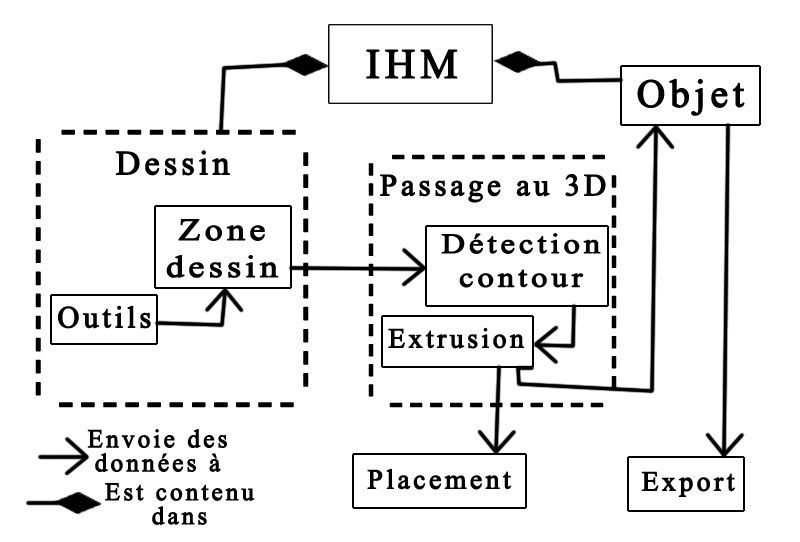
\includegraphics[scale=0.3]{images/archilogi/archi.png}}
		\begin{itemize}
			\item 
		\end{itemize}
	\end{frame}	
	
			
	\section{Etape par étape}
		%Expliquer nos choix par rapports aux objectifs énoncés
	\begin{frame}
		IHM Arnaud
	\end{frame}
	
	\begin{frame}
		Dessin -> Outils Arnaud
	\end{frame}
	
	\begin{frame}
		Dessin -> zone Etienne
	\end{frame}
	
	\begin{frame}
		Aurélien Passage au 3D
	\end{frame}
	
	\begin{frame}
		Placement Arnaud
	\end{frame}
	
	\subsection{Envoi des données}
	
	\begin{frame}{Envoi des données}
		\centerline{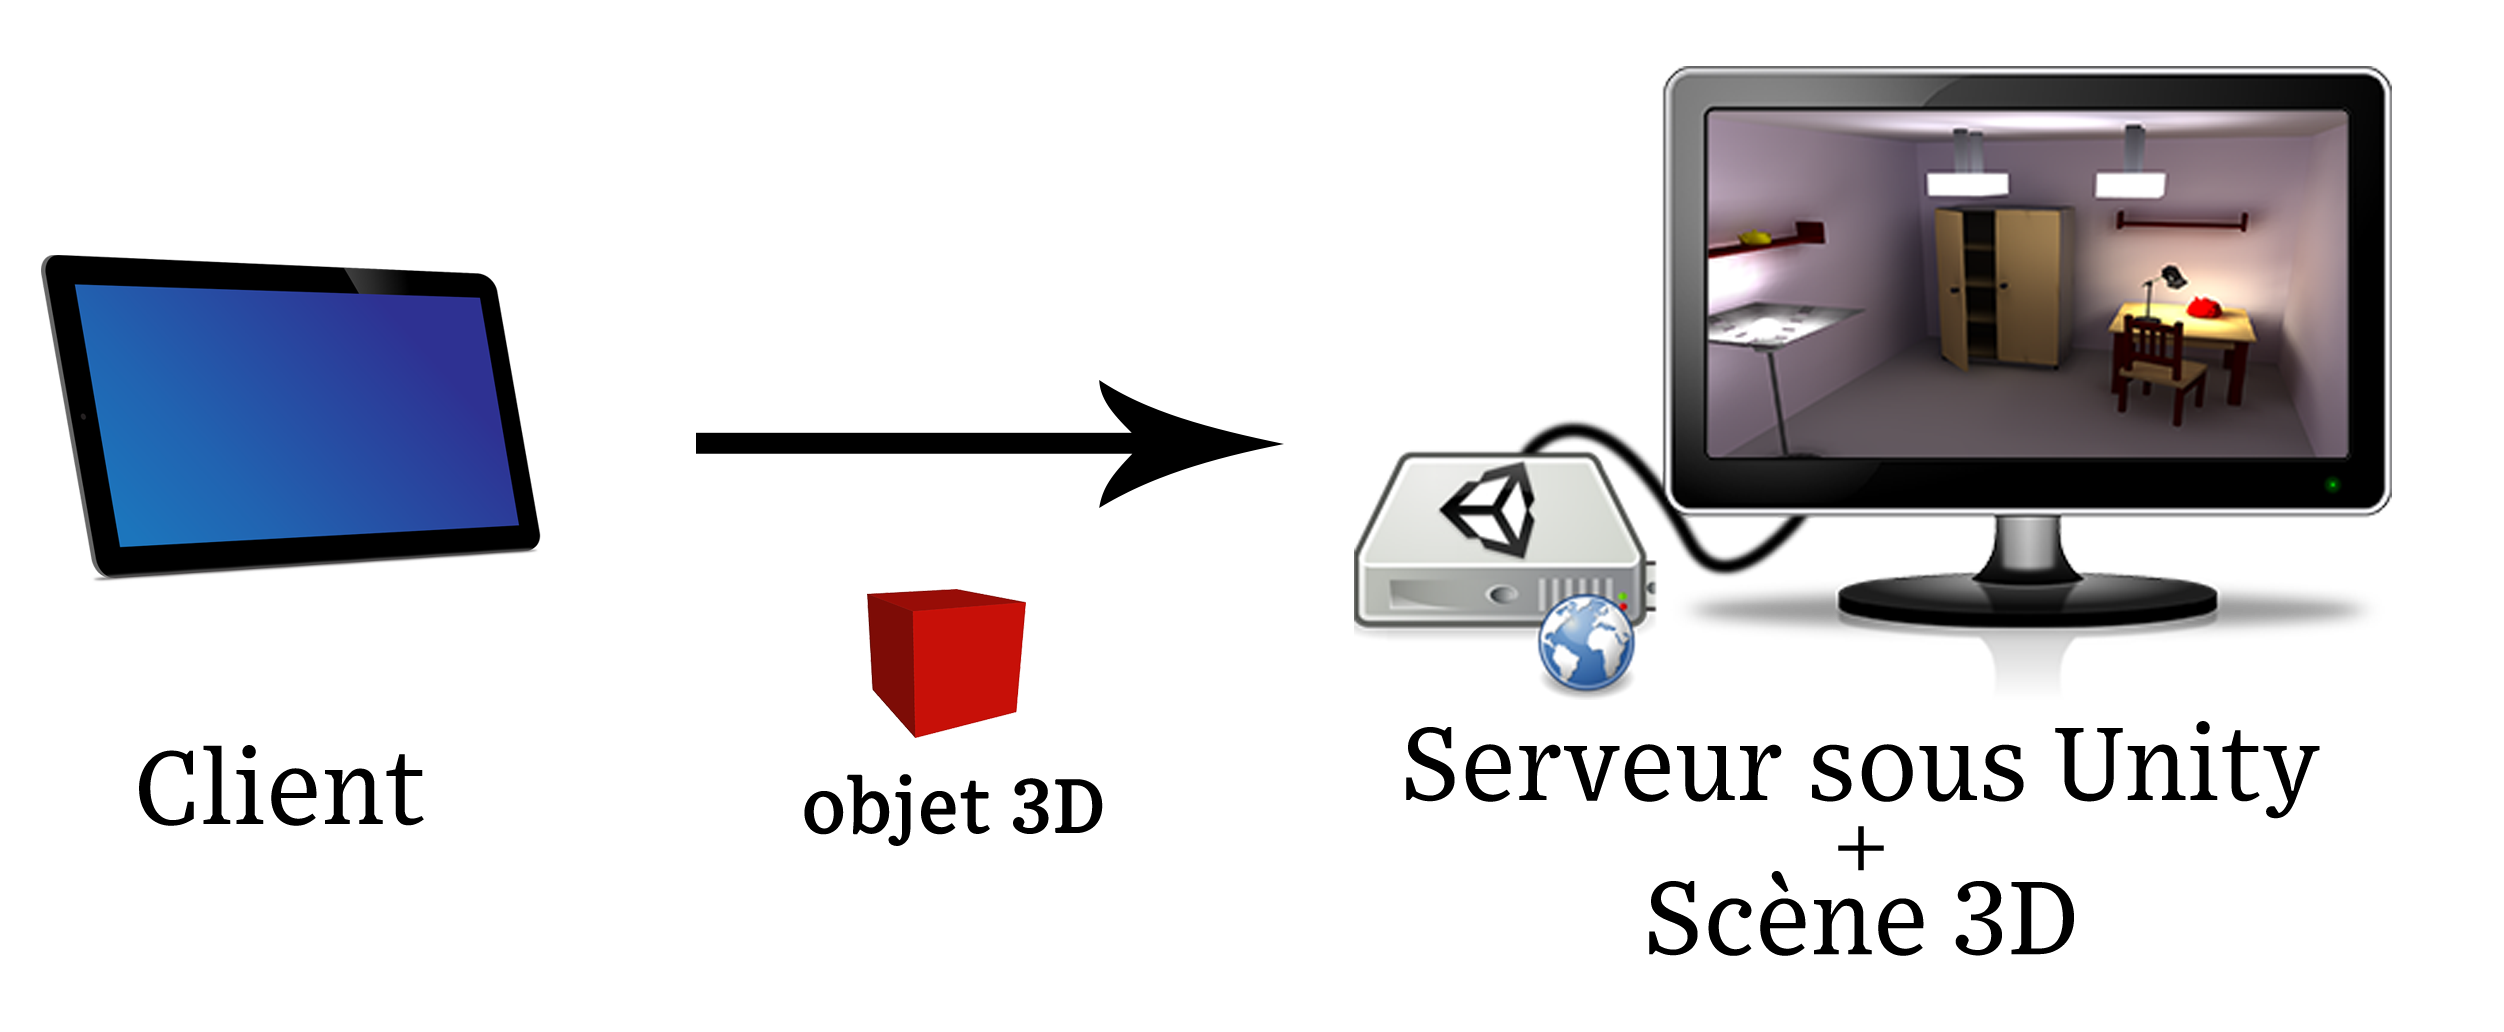
\includegraphics[height=120pt]{images/network/sending_model2.png}}
	\end{frame}
	
	\subsubsection{Côté serveur}
	
	\begin{frame}{Ajout d'un script}
		\centerline{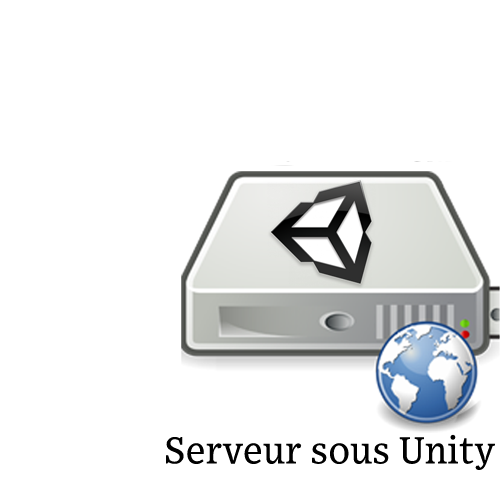
\includegraphics[height=150pt]{images/network/plugin1.png}}
		\invisible{
		\begin{itemize}	
			\item  Léger 
			\item Reçoit les données 
			\item Intégré dans la scène 3D
			\item Affiche l'objet 
		\end{itemize}	}
		
	\end{frame}
	\begin{frame}{Ajout d'un script}
		\centerline{
\includegraphics[height=150pt]{images/network/plugin.png}}
		\begin{itemize}	
			\item \pause Léger \pause
			\item Reçoit les données \pause
			\item Intégré dans la scène 3D \pause
			\item Affiche l'objet 
		\end{itemize}	
		
	\end{frame}
	
	\subsubsection{Côté client}
	
	\begin{frame}{Socket TCP}
				\centerline{\includegraphics<1>[height=120pt]{images/network/tcp-socket1.png}}
				\invisible{
					\begin{itemize}
						\item Dispose de classes prévues à cet effet en C\#
						\item Documentée en C\# par Microsoft
						\item Permet d'envoyer des octets, donc flexible
					\end{itemize}
				}
	\end{frame}
	
	\begin{frame}{Socket TCP}
		\centerline{\includegraphics<1>[height=120pt]{images/network/tcp-socket2.png}}
		\invisible{
			\begin{itemize}
				\item Dispose de classes prévues à cet effet en C\#
				\item Documentée en C\# par Microsoft
				\item Permet d'envoyer des octets, donc flexible
			\end{itemize}
		}
	\end{frame}
	\begin{frame}{Socket TCP}
		\centerline{\includegraphics<1>[height=120pt]{images/network/tcp-socket3.png}}
		\invisible{
			\begin{itemize}
				\item Dispose de classes prévues à cet effet en C\#
				\item Documentée en C\# par Microsoft
				\item Permet d'envoyer des octets, donc flexible
			\end{itemize}
		}
	\end{frame}
	\begin{frame}{Socket TCP}
		\centerline{\includegraphics<1>[height=120pt]{images/network/tcp-socket4.png}}
		\invisible{
			\begin{itemize}
				\item Dispose de classes prévues à cet effet en C\#
				\item Documentée en C\# par Microsoft
				\item Permet d'envoyer des octets, donc flexible
			\end{itemize}
		}
	\end{frame}
	\begin{frame}{Socket TCP}
		\centerline{\includegraphics<1>[height=120pt]{images/network/tcp-socket5.png}}
		\invisible{
			\begin{itemize}
				\item Dispose de classes prévues à cet effet en C\#
				\item Documentée en C\# par Microsoft
				\item Permet d'envoyer des octets, donc flexible
			\end{itemize}
		}
	\end{frame}
	\begin{frame}{Socket TCP}
		\centerline{\includegraphics<1>[height=120pt]{images/network/tcp-socket6.png}}
		\invisible{
			\begin{itemize}
				\item Dispose de classes prévues à cet effet en C\#
				\item Documentée en C\# par Microsoft
				\item Permet d'envoyer des octets, donc flexible
			\end{itemize}
		}
	\end{frame}
	\begin{frame}{Socket TCP}
		\centerline{\includegraphics<1>[height=120pt]{images/network/tcp-socket6.png}}
			\begin{itemize}
				\item Dispose de classes prévues à cet effet en C\#
				\item Documentée en C\# par Microsoft
				\item Permet d'envoyer des octets, donc flexible
			\end{itemize}
	\end{frame}
	
	\begin{frame}{Côté client}
		\centerline{\includegraphics<1>[height=140pt]{images/network/polandball_3D.png}}
	\end{frame}
	
	\section{Conclusion}
	
	\begin{frame}
		Aurélien Conclu
		%vidéo -> présente les points clés de notre présentation
	\end{frame}
		
\end{document}
